\section{Formal models of distributed system}

\subsection{Modeling}

\begin{itemize}
    \item Continuous model: described by differential equations
    \item \textbf{Discrete event models}: described by state transition systems
\end{itemize}

Modeling need to be: Complete (explain all relevant properties),
correct (behave as the system does) and Concise (explain a class of distributed
systems compactly)!

\subsubsection{State transition system (STS)}

A distributed system can be modeled as a STS. It consists of a set of initial
states, a transition function and a set of states. Informally, the transition
function describes the allowed state of the system after some event in the previous
state.

\begin{enumerate}
    \item[$\to$] like finite state machine but no input needed
\end{enumerate}

\begin{itemize}
    \item A \textbf{configuration} is a snapshot of state of all node

        $$ C =(q_0, q_1, q_2,\ldots, q_{n-1}) $$  where $q_i$ is state of node $p_i$.
\end{itemize}

\paragraph{Property}
Determinism, I/O and atomicity.

\subsubsection{Node}
Can send, receive messages and do local computations. Nodes are deterministic
(I/O is in the node) and atomic (no I/O during computations). All non determinism
comes from the delivery of messages.

A node state is defined by triple $<I, O, s>$:
\begin{itemize}
    \item $l$: inbuffer set for each neighbor (vector)
    \item $O$: outbuffer set for each neighbor (vector)
    \item $s$: local state
\end{itemize}

\begin{figure}[!ht]
    \centering
    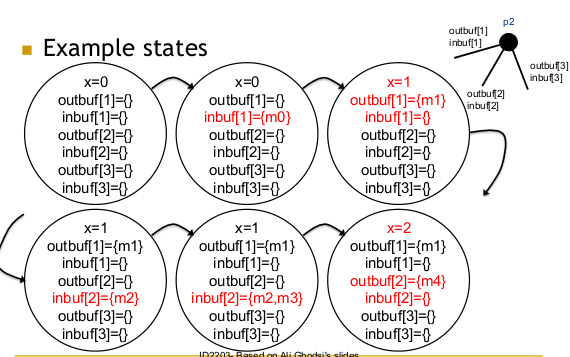
\includegraphics[width=10cm]{img/node.png}
    \caption{Example states}
\end{figure}
\FloatBarrier{}

\paragraph{Working}
\begin{enumerate}
    \item Wait for message
    \item When receive message, do some computation and send message
    \item Goto 1.
\end{enumerate}

\paragraph{Events}
\begin{itemize}
    \item $comp(i)$: computation event at process $i$.
        \subitem{} \textit{Apply transition function $f$ on node $i$ state}
    \item $del(i, j, m)$: delivery event of msg $m$ from $i$ to $j$
        \subitem{} \textit{Move $m$ from outbuf of $p_i$ to inbuf $p_j$}
\end{itemize}

\subsubsection{Transition functions}

Formally a transaction functions requires for any two
$f(<I_1,O_1,s_f1>)=<I_2,O_2,s_2>$ and $f(<I_3,O_3,s_3>)=<I_4,O_4,s_4>$
\begin{itemize}
	\item $I_2=I_4 =<\emptyset,\ldots,\emptyset>$ (all inbufs are empty)
	\item if $I_2=I_4$ and $s_1=s_3$ then
	\begin{itemize}
		\item $s_2=s_4$ (don't observe channel)
		\item $O_1[i] \subseteq O_2[i]$ and $O_3[i] \subseteq O_4[i]$
		(only add msg to outbuf)
		\item $O_2[i]-O_1[i] = O_4[i]-O_3[i]$ (don't observe channel)
	\end{itemize}
\end{itemize}

You can denote it \verb#app(e,c)# with $e$ an event and $c$ a configuration.

\subsubsection{Execution}
An execution is a infinite sequence of \enquote{$config_0, event_1, config_1,
event_2, config_2,\cdots$}


\begin{itemize}
    \item[If] $event_k = comp(i)$: $config_{k-1}$ change to $config_k$
        by applying $p_i$'s transition function on i's state in
        $config_{k-1}$
    \item[If] $event_k = del(i, j, m)$: $config_{k-1}$ change to $config_k$
        by moving m from i's outbuf to j's inbuf
\end{itemize}


\subsubsection{Property}

\begin{itemize}
    \item For each $comp(i)$ is associated a \textbf{transition} $(state_1, state_2, i)$
    \item Transition $(s_1, s_2, j)$ is \textbf{applicable} in
        configuration $c$ if accessible state of node $j$ in $c$ is $s_1$
    \item $del(i, j, m)$ \textbf{application} in configuration $c$ if $m$ is
        in outbuf for link $i \leftrightarrow j$ of node $i$ in $c$

        %TODO EXAMPLE SLIDE 11?

    \item \begin{enumerate}
            \item if transition $e=(s_1, s_2, i)$ is applicable
            \item or if $e=del(i, j, m)$ is applicable
        \end{enumerate}
        to configuration $c$, then $app(e,c)$ is the new configuration after
        the event $comp(i)$ or $del(i,j,m)$

\end{itemize}


\subsection{Asynchronous (Schedules) / Synchronous}
Processes are deterministic,
Non-determinism comes from asynchrony (messages take arbitrary time to
be delivered, and the time to compute varies)\ldots \newline

A \textbf{schedule} is the sequence of events. The event are the
one that determine the properties $(del(i,j,m)$ determines the message
asynchrony and $comp(i)$ determines the proccess speed.)
 so all non-determinism is embedded in schedule.

\begin{itemize}
	 \item Given the initial conf, the schedule determines the whole
	 execution.
	 \item Not all schedules are allowed for initial conf. (some
	 event may be impossible to occurs)
\end{itemize}

\subsection{Order of event}
The order in which two applicable computation events or
two applicable delivery events are executed is irrelevant!\\
The idea of the proof is that if you two differents comp
events $a$ and $b$ (meaning on different node!) applicable in a
configuration then appliying $a$ first will not change the state of the
node related to $b$ (vice-versa).
\paragraph{Note} It is only true for event that are not causally
related!
\subsection{Admissible execution (Fairness)}
An execution is admissible if:
\begin{itemize}
	\item Each process has infinite number of $comp(i)$;
	\item Every message m sent is eventually $del(i,j,m)$.
\end{itemize}
The infinity property permit messages to wait arbitrary long times before
being delivered.
\subsection{Synchronous Systems}
The execution is partitionned into disjoint rounds. A round consists of
deliver event for all messages in outbuf and one compute event on
every process.

\subsubsection{Causal order $<_H$}
Causal order is \textbf{transitive}.

\begin{itemize}
    \item[$ a <_H b $]
    \item if $a$ occurs before $b$ on the same process
    \item if $a$ produces $m$ and $b$ delivers $m$
    \item if $a$ delivers $m$ and $b$ consumes $m$
\end{itemize}

\paragraph{Concurrent}
$a$ and $b$ are concurrent (denoted $a || b$), if not $a <_H b$ and not $b <_H a$

\subsection{Similarity of execution}
\begin{itemize}
	\item The view of $p_i$ in $E$, denoted $E|p_i$ is the subsequence
	of executions E restricted to events and state $p_i$.
	\item 2 executions E,F are similar w.r.r if E|$p_i$ = F|$p_i$.
\end{itemize}
\paragraph{Computation Theorem}
\begin{itemize}
	\item Let $E$ an execution ($c_0,e_1,c_1,e_2,\ldots$) and V the
	schedule of event ($e_1,e_2,e_3,\ldots$) s.t. $app(e_i,c_{i-1})=c_i$
	\item Let $P$ be a permutation of V preserving casual order.
\end{itemize}
Then $E$ is similar to the execution starting in $c_0$ with schedule $P$.
\subparagraph{Notations}

Similar executions $E$, $F$ are denoted F\textasciitilde{}E.
\begin{description}
	\item[Computations or Equivalence class:] A class s.t all the elements
are similar to each other.
\end{description}
Computation theorem implies two importants results:
\begin{enumerate}
	\item There is no algorithm that can observe the order of the sequence
	of events for all executions. %TODO ADD PROOF (pas compris)
	\item Computation theorem does not hold in a model extended s.t each
	process read an hardware clock.%%TODO ADD PROOF (pas compris)
\end{enumerate}
\subsection{Clock}
A clock is used to tell locally if two events are causally related.

\subsubsection{Lamport Clock}
\begin{itemize}
    \item Each process has a local logical clock, $t$ initially $t=0$.
        Node $p$ piggyback $(t, p)$ on every sent message.
    \item On each event:
    \begin{enumerate}
        \item $t = \max(t, t_q) + 1$: when $p$ receives message with
            timestamp ($t_q, q$) (delivery from $q$)
        \item $t = t+1$: for every transistion (comp)
    \end{enumerate}

    \item[$\to$]
        \begin{itemize}
            \item $(t_p, q) < (t_q, q)$ IFF $(t_p <t_q \vee (t_p = t_q \wedge p <
        q))$
\end{itemize}
\end{itemize}

Lamport logical clock guarantee that if $a <_H b$, then $t(a) < t(b)$

\subsubsection{Vector clock}
\begin{itemize}
    \item Each process has a local vector, $v_p$ of size $n$. Initially
        $\forall i : v_p[i]=0$

        Node $p$ piggyback $v_p$ on every sent message.
    \item On each event:
    \begin{enumerate}
        \item $v_p[p] = v_p[p] + 1$
        \item $\forall_i : v_p[i] = \max(v_p[i], v_q[i])$
    \end{enumerate}

\item[$\to$] \begin{itemize}
        \item $v_p \leq v_q$ iff $\forall_i : v_p[i] \leq v_q[i]$
        \item $v_p < v_q$ iff $v_p \leq v_q$ and $\exists i : v_p[i] <
            v_q[i]$
        \item $v_p$ and $v_q$ are concurrent (denoted $v_p \mid\mid v_q$) iff
        $\lnot(v_p < v_q) \land \lnot(v_q < v_p)$
    \end{itemize}
\end{itemize}

Vector clock guarantee that if $v(a) < v(b)$ then $a <_H b$ but also if
$a <_H b$ then $v(a) < v(b)$

\subparagraph{Precisions}
Vector clock cannot be done with smaller vector than size $n$ for $n$ nodes
\begin{itemize}
	\item The relation $<_H$ is a partial order (no ordering of concurrent events)
	\item The relation $<$ on Lamport logical clock is a total order (ordering of clock values)
	\item The relation $<$ on vector timestamps is a partial order (no ordering on TS of concurrent events)
\end{itemize}

\subsection{Complexity}
Defined over the
\begin{itemize}
	\item Number of messages used before terminating
	\item Time it takes to terminate
\end{itemize}
An algorithm has terminated when all states in a config. are terminated
states and there is no more messages in (in/out)bufs.\\
\paragraph{Time Complexity}
A message delay is at most 1 time unit while a computation events take
0 time units. A \textbf{timed execution} is an execution s.t
\begin{itemize}
	\item Time is associated with each $comp(i)$ event
	\item First event happens at time $0$
	\item Time can never decrease and strictly increases locally.
	\item Max time between $comp(i)$ sending $m$ and $comp(j)$
	consuming $m$ is $1$ time unit.
\end{itemize}
Time complexity is maximum time until termination for all
admissible timed executions.
